\documentclass[10pt]{article}

\usepackage{graphicx}
\usepackage{amsmath,amsfonts,amssymb}

\usepackage{hyperref}  % for urls and hyperlinks


\setlength{\textwidth}{6.2in}
\setlength{\oddsidemargin}{0.3in}
\setlength{\evensidemargin}{0in}
\setlength{\textheight}{8.9in}
\setlength{\voffset}{-1in}
\setlength{\headsep}{26pt}
\setlength{\parindent}{0pt}
\setlength{\parskip}{5pt}




% a few handy macros

\newcommand\matlab{{\sc matlab}}
\newcommand{\goto}{\rightarrow}
\newcommand{\bigo}{{\mathcal O}}
\newcommand{\half}{\frac{1}{2}}
%\newcommand\implies{\quad\Longrightarrow\quad}
\newcommand\reals{{{\rm l} \kern -.15em {\rm R} }}
\newcommand\complex{{\raisebox{.043ex}{\rule{0.07em}{1.56ex}} \hskip -.35em {\rm C}}}


% macros for matrices/vectors:

% matrix environment for vectors or matrices where elements are centered
\newenvironment{mat}{\left[\begin{array}{ccccccccccccccc}}{\end{array}\right]}
\newcommand\bcm{\begin{mat}}
\newcommand\ecm{\end{mat}}

% matrix environment for vectors or matrices where elements are right justifvied
\newenvironment{rmat}{\left[\begin{array}{rrrrrrrrrrrrr}}{\end{array}\right]}
\newcommand\brm{\begin{rmat}}
\newcommand\erm{\end{rmat}}

% for left brace and a set of choices
\newenvironment{choices}{\left\{ \begin{array}{ll}}{\end{array}\right.}
\newcommand\when{&\text{if~}}
\newcommand\otherwise{&\text{otherwise}}
% sample usage:
%  \delta_{ij} = \begin{choices} 1 \when i=j, \\ 0 \otherwise \end{choices}


% for labeling and referencing equations:
\newcommand{\eql}{\begin{equation}\label}
\newcommand{\eqn}[1]{(\ref{#1})}
% can then do
%  \eql{eqnlabel}
%  ...
%  \end{equation}
% and refer to it as equation \eqn{eqnlabel}.  


% some useful macros for finite difference methods:
\newcommand\unp{U^{n+1}}
\newcommand\unm{U^{n-1}}

% for chemical reactions:
\newcommand{\react}[1]{\stackrel{K_{#1}}{\rightarrow}}
\newcommand{\reactb}[2]{\stackrel{K_{#1}}{~\stackrel{\rightleftharpoons}
   {\scriptstyle K_{#2}}}~}

% Parts:

% set enumerate to give parts a, b, c, ...  rather than numbers 1, 2, 3...
\renewcommand{\theenumi}{\alph{enumi}}
\renewcommand{\labelenumi}{(\theenumi)}

% set second level enumerate to give parts i, ii, iii, iv, etc.
\renewcommand{\theenumii}{\roman{enumii}}
\renewcommand{\labelenumii}{(\theenumii)}

  % input some useful macros

\begin{document}

% header:
\hfill\vbox{\hbox{AMath 585}
\hbox{Homework \#4}\hbox{Due Thursday, February 20, 2020}}

\vskip 5pt

Homework is due to Canvas by 11:00pm PDT on the due date.

To submit, see
\url{https://canvas.uw.edu/courses/1352870/assignments/5253097}





%--------------------------------------------------------------------------
\vskip 1cm
\hrule
{\bf Preamble.}
Recall that ``spectral accuracy'' often means the error decays faster than
any algebraic power of $N^{-1}$ as we increase
the number of points $N$ used in our approximation.

Recall that if the error (in e.g. the max-norm) behaves like 
$E(N) \approx C N^{-p}$
as $N \goto \infty$ then $\log E(N) \approx \log(C) - p\log(N)$ so we expect
the slope to be $-p$ if we do a log-log plot of $E(N)$ vs. $N$.
If we are seeing spectral accuracy then we expect the slope to keep
decreasing as $N$ grows, until rounding errors take over.

Sometimes we have even better accuracy than this suggests, and in fact 
$E(N) \approx C \exp(-\gamma N)$ for some constants $C, \gamma > 0$.  This
means the error is decaying exponentially fast with $N$ (which in particular
is faster than any algebraic power, but there are things in between).

If we have exponential convergence then we expect $\log(E(N)) \approx
\log(C) -\gamma N$.  Note that we now have $N$ not $\log(N)$ on the right
and so this looks linear in a semilogy plot in which we plot $\log(E(N))$
vs. $N$ itself (e.g. using the {\tt semilogy} command in Matlab or Python.
The slope in such a plot shows the decay rate $\gamma$.  

Here's a comparison of these two plots for the case of the Runge function
$u(x) = 1/(1 + 16x^2)$ with interpolation at $N$ Chebyshev points.

\hfil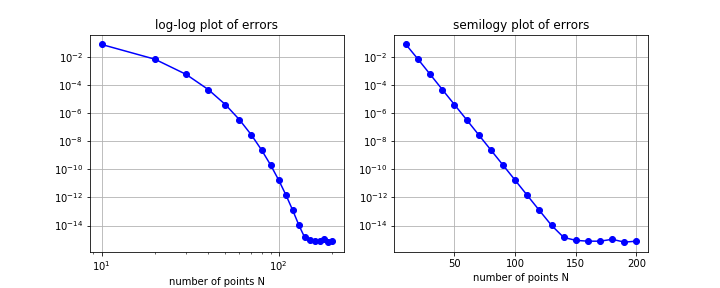
\includegraphics[width=5.5in]{RungeErrors.png}\hfil

We see exponential convergence!



%--------------------------------------------------------------------------
\vskip 1cm
\hrule
{\bf Problem 1.}
(a) Adapt the code from the {\tt ChebyshevSpectral.ipynb} notebook to reproduce
these figures.  Use the max-norm of the error, approximated by 
evaluating the interpolating polynomial at 1000 points and comparing to the
original function at these points.

(b) Change to this variant of the Runge function: $u(x) = 1/(1 + 25x^2)$,
which is also commonly used.  This function has poles at $\pm 0.2i$ in the
complex plane, closer to the real axis than the previous function.  As a
result the convernence is not quite as fast, though still exponential.
Make these plots.

It can be shown that the convergence is exponential provided the
extension of the function $u(x)$ to the complex plane is analytic near the
real axis, and the rate depends on how far out it is analytic.

(c) If the function is analytic in the entire complex plane then convergence is
even faster than exponential, meaning the slope continues to decrease even
in a semilogy plot.  

Illustrate this for $u(x) = (x-0.5)\sin(10x)$, 
using smaller values of $N$ since convergence is so fast!

See e.g. Trefethen's books if you want to read more about this.

% uncomment the next two lines if you want to insert solution...
%\vskip 1cm
%{\bf Solution:}

% insert your solution here!

%--------------------------------------------------------------------------
\vskip 1cm
\hrule
{\bf Problem 2.}
The notebook {\tt ChebyshevSpectral.ipynb} illustrates how to approximate
$u'(x)$ by doing Chebyshev polynomial interpolation to get $p(x)$ and then
computing $p'(x)$.  Extend this to give an approximation to $u''(x)$ by
computing $p''(x)$.  You will have to write a function to compute $T_n''(x)$
for each basis function $T_n(x)$, similar to what was done for $T_n'(x)$.

Test this out by computing the second derivative of these functions, and
also produce semilogy plots of the errors as $N$ is increased:

\begin{itemize}
\item $u(x) = \sin(2x),$
\item $u(x) = (x-0.5)\sin(10x),$
\item $u(x) = 1/(1 + 16x^2).$
\end{itemize}
Comment on any interesting behavior you observe.

% uncomment the next two lines if you want to insert solution...
%\vskip 1cm
%{\bf Solution:}

% insert your solution here!


%--------------------------------------------------------------------------
\vskip 1cm
\hrule
{\bf Problem 3.}

Now write a routine to solve the Boundary value problem
\[
u''(x) = f(x), \quad -1\leq x \leq 1,
\]
with Dirichlet boundary conditions $u(-1)=\alpha, ~ u(1)=\beta$, using
spectral collocation at the Chebyshev points.

Test it out at least on the case where the true solution is $u(x) =
\sin(2x)$ (which defines $f(x)$ and the boundary values)
and produce a semilogy plot of the errors.

{\bf Hints:} You need to set up and solve a linear system of equations for
the coefficients $c_n$ in the polynomial
\[
p(x) = \sum_{n=0}^N c_n T_n(x).
\]
The equations in the system include the boundary conditions,
\[
\sum_{n=0}^N c_n T_n(-1) = \alpha, \quad 
\sum_{n=0}^N c_n T_n(1) = \beta,
\]
and then the collocation equation at each interior node ($j=1,2,\ldots,N-1$):
\[
\sum_{n=0}^N c_n T_n''(x_j) = f(x_j).
\]
Recall also that if you define $x_j = \cos(j \pi/N)$ then these are ordered from
right to left with $x_0=1$ and $x_N=-1$.

% uncomment the next two lines if you want to insert solution...
%\vskip 1cm
%{\bf Solution:}

% insert your solution here!


%--------------------------------------------------------------------------

\end{document}
